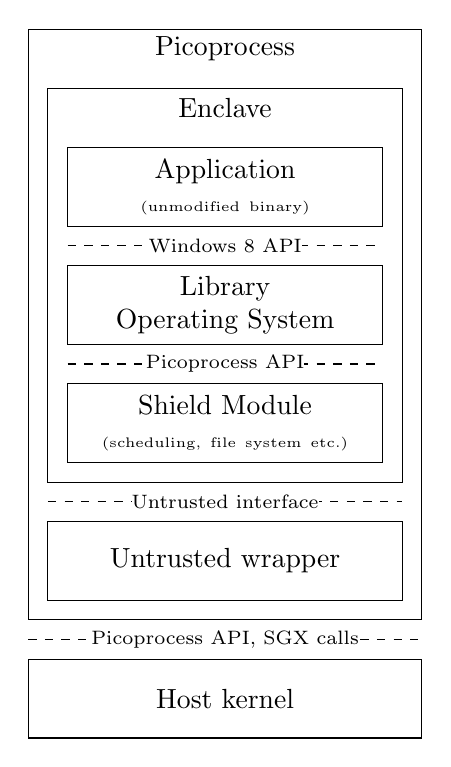
\begin{tikzpicture}[
    x=1cm,y=1cm,
	block/.style={draw, text width=4cm, minimum height=1cm, align=center, inner sep=0},
	label/.style={midway, font=\scriptsize, fill=white, inner sep=0}
]

\node[block] at (0,0) {Application\\\tiny(unmodified binary)};
\draw[dashed]  (-2,-0.75) -- (2,-0.75) node [label] {Windows 8 API};
\node[block] at (0,-1.5) {Library\\Operating System};
\draw[dashed]  (-2,-2.25) -- (2,-2.25) node [label] {Picoprocess API};
\node[block] at (0,-3) {Shield Module\\\tiny(scheduling, file system etc.)};

\node at (0,1) {Enclave};
\draw  (-2.25,1.25) rectangle (2.25,-3.75);
\draw[dashed]  (-2.25,-4) -- (2.25,-4) node [label] {Untrusted interface};
\node[block, text width=4.5cm] at (0,-4.75) {Untrusted wrapper};

\node at (0,1.75) {Picoprocess};
\draw  (-2.5,2) rectangle (2.5,-5.5);
\draw[dashed]  (-2.5,-5.75) -- (2.5,-5.75) node [label] {Picoprocess API, SGX calls};

\node[block, text width=5cm] at (0,-6.5) {Host kernel};
\end{tikzpicture}